\documentclass[10pt]{article}
 
\usepackage[a4paper, 
 	width = 170mm,
 	height = 270mm]{geometry}

\usepackage{color}
\definecolor{SU}{RGB}{0, 46, 95}

\usepackage{booktabs}
\usepackage{graphicx}

\usepackage{microtype}
 	
\usepackage{hyperref}
\hypersetup{
 	colorlinks,
 	citecolor = black,
 	filecolor = black,
 	linkcolor = SU,
 	urlcolor = SU,
 	pdfauthor = {Leonard Blaschek},
 	pdftitle = {phenotyping guide},
 	pdfkeywords = {Lignin methods}
}
 
\title{Guidelines for image based phenotyping of \textit{A. thaliana}}
 
\author{Leonard Blaschek}
 
\begin{document}
 	\maketitle
 	
 	\section*{Why we use image based phenotyping}
 	
	We perform image based automated phenotyping to measure more parameters of plant growth at a higher temporal resolution than we could feasibly do using manual methods. Not only do image based approaches allow us to measure plants' height, area, colour and overall shape throughout their life cycle, the high quality images themselves can be used to measure additional features or phenotypes later on. As with all image analysis approaches, the quality of the input images is the single most important variable in determining success. In the approach implemented by me, two imaging setups are used, depending on the developmental stage of the \textit{A. thaliana} plants.

 	\section{Rosette growth}
 	
 	From germination until bolting, the plants are best imaged from the top. One big advantage of this is that the pots can be left in the tray, meaning that 15 plants can be analysed from a single picture. As you can see from the example image in figure \ref{fig:top}, I acquire the images without labels. Instead, I have labels on the side of the pots (see figure \ref{fig:front_before}). That of course means that you have to be very careful to document the order of pots (genotypes/replicates) in each tray, and orient the trays in the same way in each picture (put a label on one side of the tray to make sure you do not accidentally flip it 180°). You also need to carefully document which picture shows which tray. Lastly, bright markers (any colour that stands out, I use light blue) on the outer edges of the tray allow you to easily crop the image to the area of interest in the analysis.
 	
 	\begin{figure}[!h]
 		\centering
 		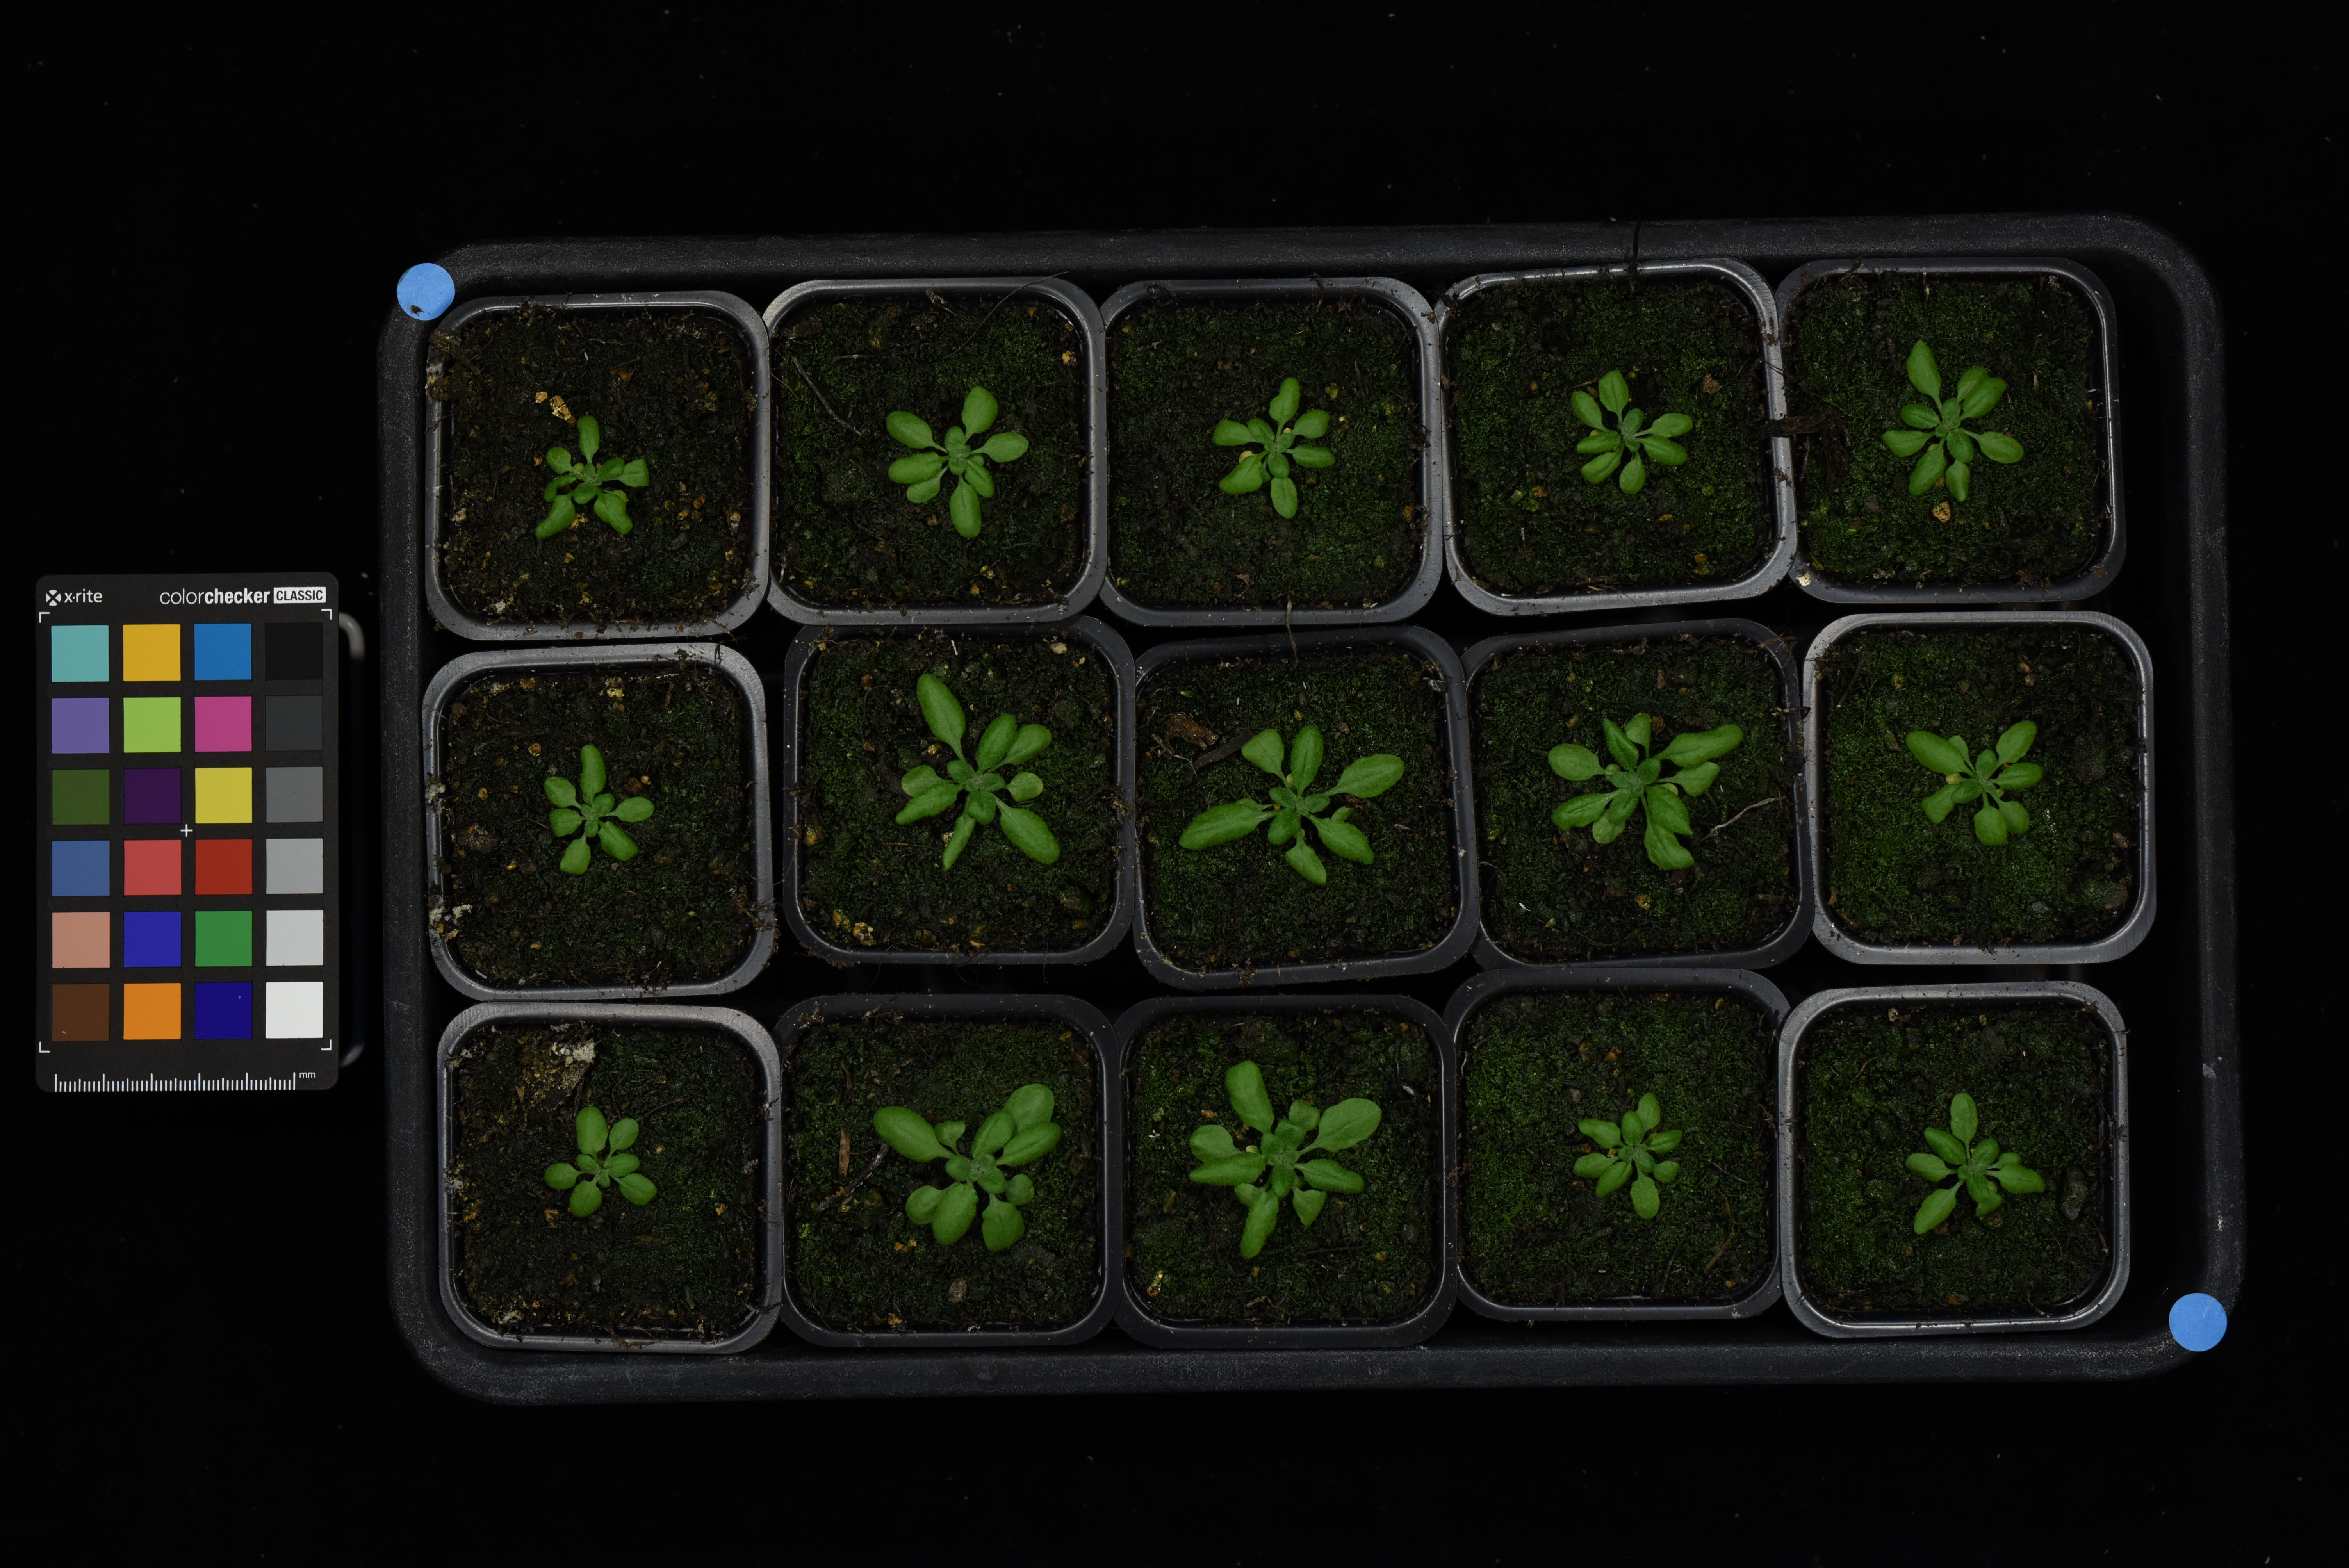
\includegraphics[width=0.5\linewidth]{21_1}
 		\caption[Example image of a top-view image.]{\textit{A. thaliana} plants during their vegetative phase (before bolting of the inflorescence stem), imaged from the top. The image should cover the whole tray and the colour card to the left, both of which should be oriented in parallel with the image borders. Acquisition parameters need to be chosen to avoid over-exposure. Also note the blue stickers on the corners of the tray, which are later used to define the area of interest for the image analysis.}
 		\label{fig:top}
 	\end{figure}
 
 	\noindent In order to avoid over-exposure, the following acquisition parameters have proven successful in our setup:
 
	 \begin{itemize}
	 	\item 50 mm objective
	 	\item 1/125 s exposure time
	 	\item f5.6 aperture
	 	\item 800 ISO sensitivity
	 	\item white balance set to "Incandescent"
	 \end{itemize}
 
 	\section{Inflorescence growth}
 	
 	After the plants bolt, we switch to imaging from the front. Now we have to image each plant individually. Make sure that the label on the front of the pot is clearly visible in each image. Everything in the image that is \textit{not} the plant or the colour card, such as labels, sticks, pots, \textit{etc.} should be of a colour that is easy to distinguish from the plant. Because \textit{A. thaliana} can be green (leaves), white (flowers), purple (stressed leaves), yellow/beige/brown (plants in senescence), the ideal colour for foreign objects is blue (see stick in figure \ref{fig:front_after}).
 	
 	\begin{figure}[!h]
 		\centering
 		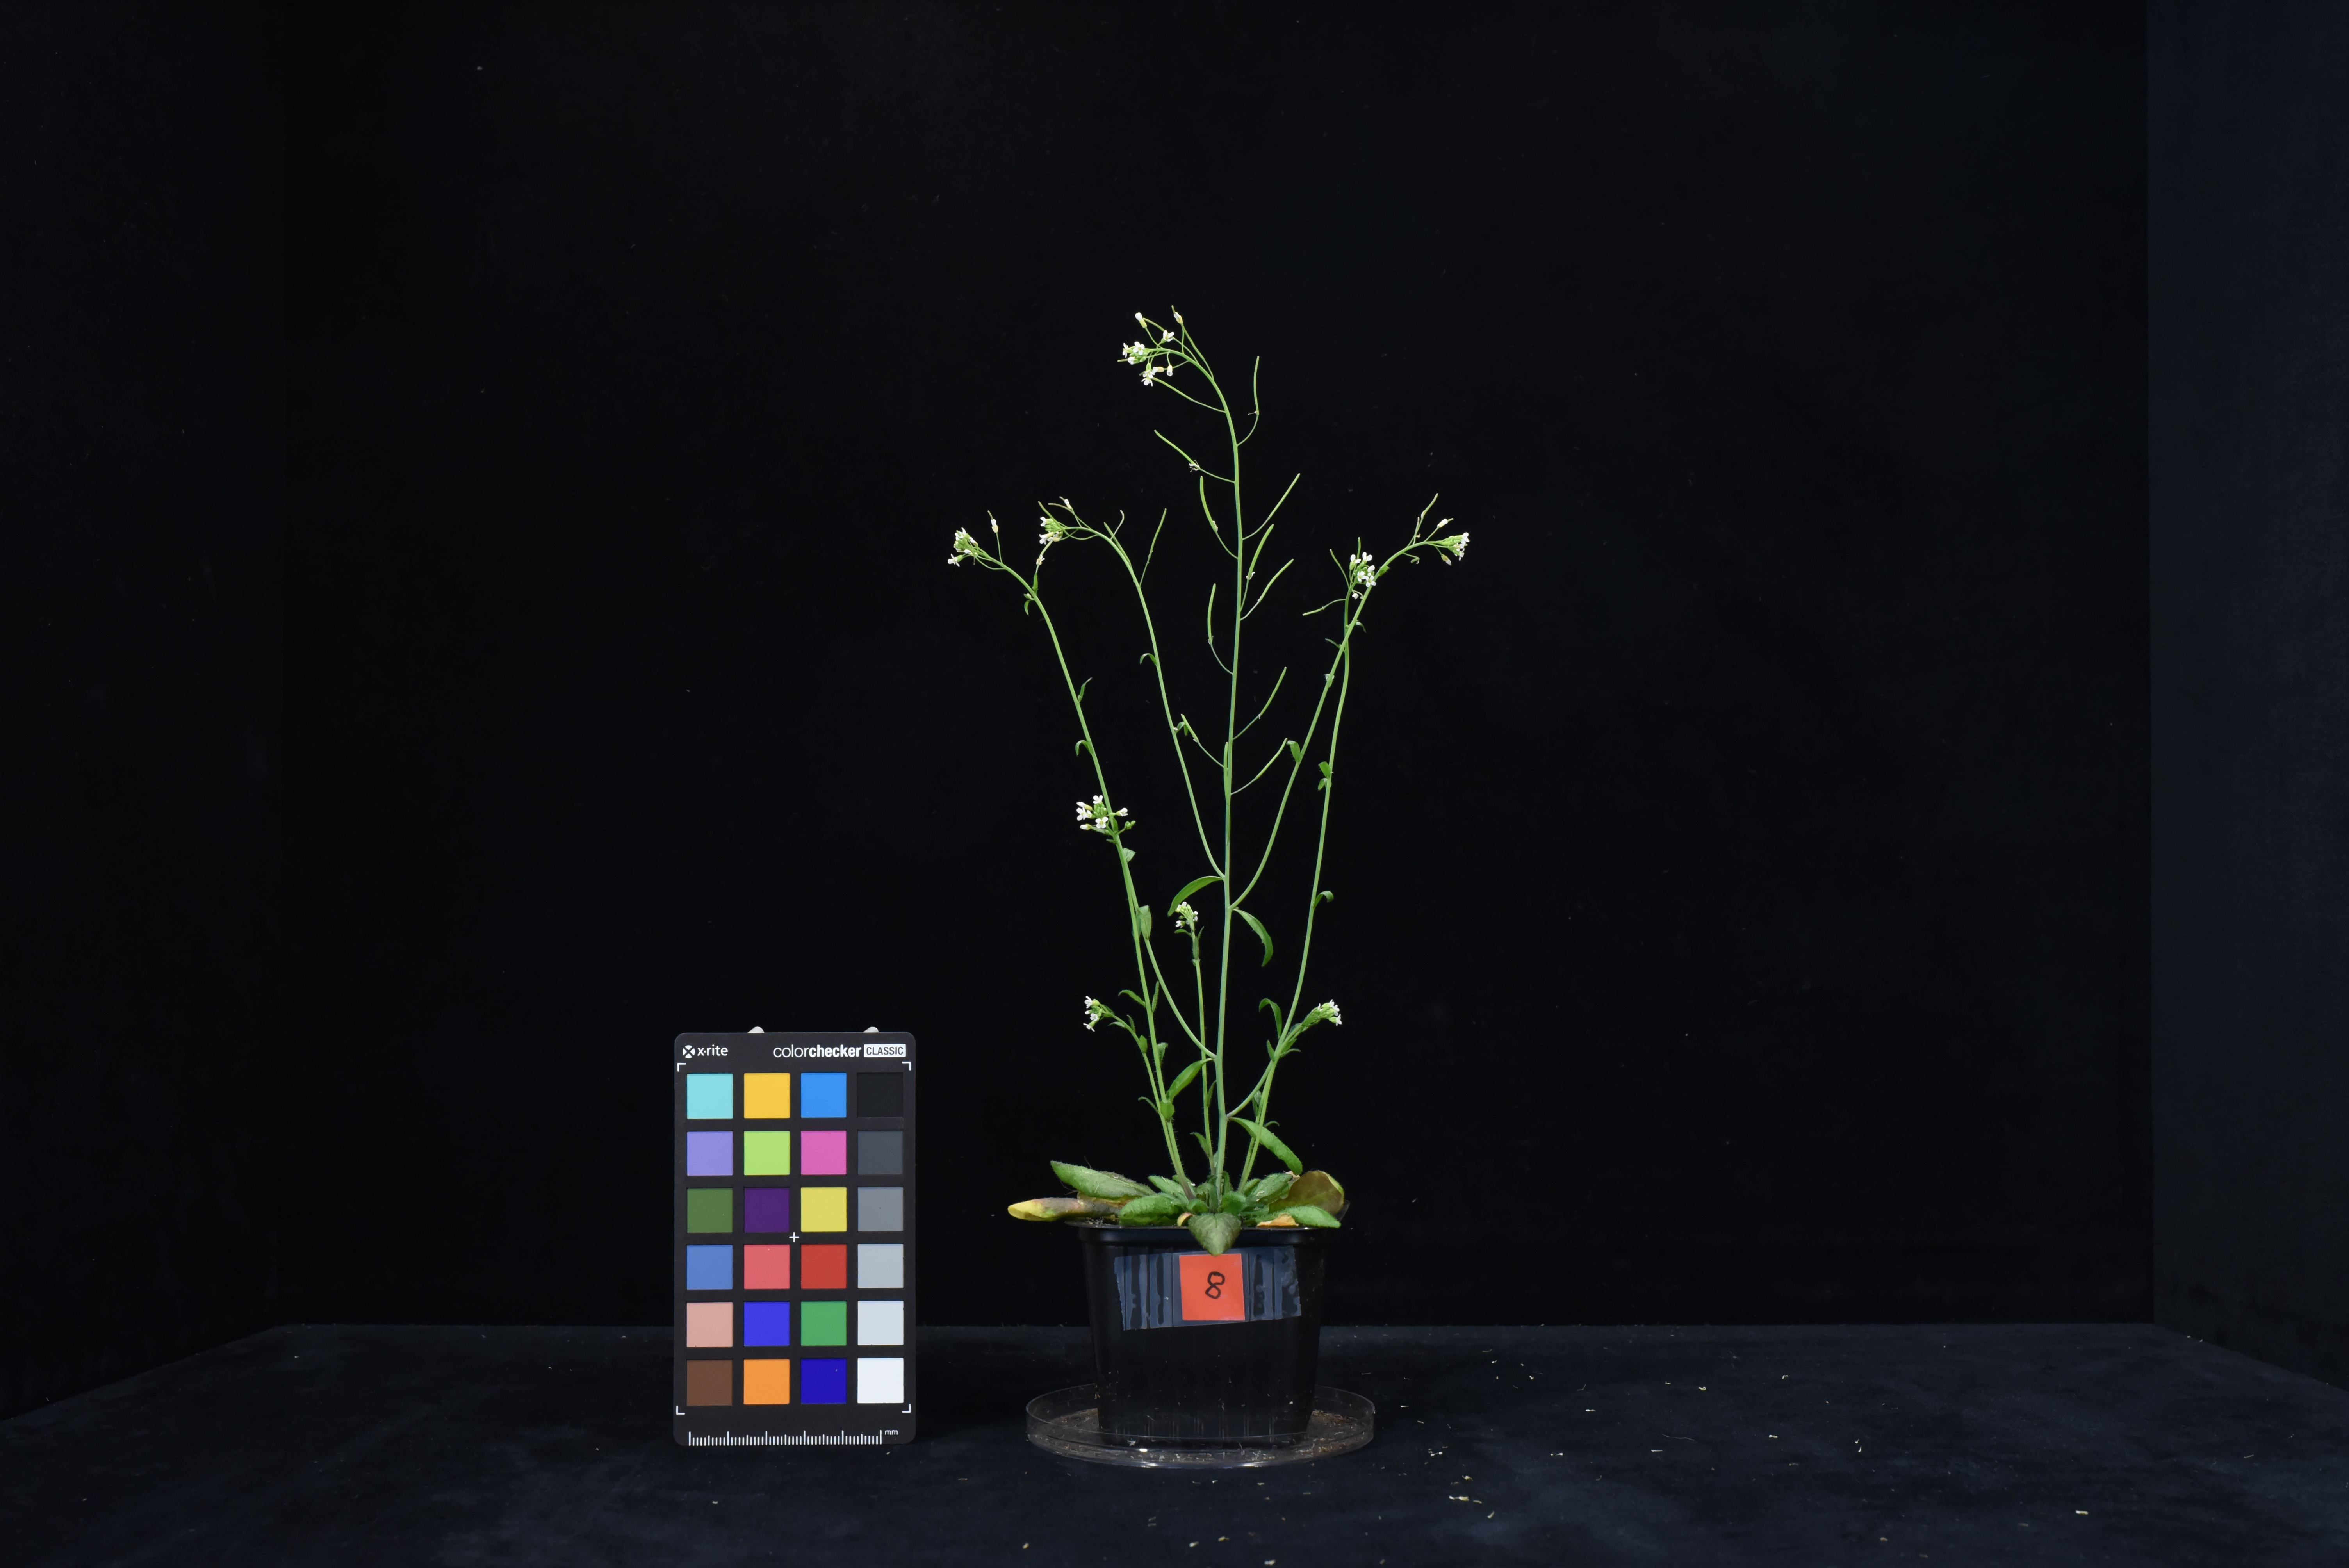
\includegraphics[width=0.5\linewidth]{20201008_8}
 		\caption[Example image of a front-view image.]{An \textit{A. thaliana} plant during its reproductive phase (after bolting of the influorescence stem, but \textbf{before} binding the stems to a stick), imaged from the front. The image should cover the whole plant and the colour card to the left, both of which should be oriented in parallel with the image borders. Acquisition parameters need to be chosen to avoid over-exposure. Also note the red label on the front of the pot, used for identification. This label can contain any amount of text, but should be blue or red, to avoid colour similarity to the plant itself.}
 		\label{fig:front_before}
 	\end{figure}
 
 	\noindent For this stage, the following acquisition parameters have proven successful in our setup:
 	
 	\begin{itemize}
 		\item 50 mm objective
 		\item 1/30 s exposure time
 		\item f13 aperture
 		\item 2000 ISO sensitivity
 		\item white balance set to "Incandescent"
 	\end{itemize}
 
	 \begin{figure}[!h]
	 	\centering
	 	\includegraphics[width=0.3\linewidth]{20201029_8}
	 	\caption[Example image of a front-view image.]{An \textit{A. thaliana} plant during its reproductive phase (\textbf{after} binding the stems to a stick), imaged from the front. Just like the label, the stick should ideally be blue to facilitate separation from the plant itself in the analysis.}
	 	\label{fig:front_after}
	 \end{figure}
 
 \section{Analysis}
 
 Depending on preferences and coding experience, these images can be analysed using a range of different approaches from fully manual to fully automated.
 
 \subsection{Fiji}
 
 To get a feeling for the images, open one of them in \href{https://imagej.net/Fiji/Downloads}{Fiji} and explore how you can segment and measure different parts of the plant. A very useful function for this is \texttt{Image} $\rightarrow$ \texttt{Adjust} $\rightarrow$ \texttt{Color Threshold...} (use the LAB colour space). To calibrate any height or area measurements, you can define the pixel size using the ruler on the bottom of the colour card.
 
 \subsection{Python and PlantCV}
 
 You can do the complete analysis in Fiji, but depending on the amount of images you have, this might be prohibitively time consuming. The alternative is to automate the same principles of image analysis that we would use in Fiji, using the python library \href{https://plantcv.danforthcenter.org/}{PlantCV}. The official \href{https://plantcv.readthedocs.io/en/stable/}{documentation} of Plant CV does a much better job of introducing the software and getting you started with simple workflows than I ever could. Once you have acquainted yourself with the software, the analysis scripts that I optimised for our system are available on my \href{https://github.com/leonardblaschek/plantcv}{Github page}.
 	
 	
\end{document}
